\documentclass[pdf, aspectratio=169, 12pt]{beamer}
\usepackage[]{hyperref, graphicx, siunitx, lmodern, tikz, booktabs, physics}
\usepackage[mode=buildnew]{standalone}
\usepackage{pdfpc-commands}

\usetheme{Python}

\sisetup{per-mode=symbol}
\usetikzlibrary{calc, patterns, decorations.markings, decorations.pathmorphing, shapes}

%Preamble
\title{Becoming a Parseltongue}
\author{Jed Rembold}
\date{January 22, 2020}

\begin{document}
%\renewcommand{\theenumi}{\Alph{enumi}}

\begin{frame}{Announcements}
	\begin{itemize}
		\item Welcome to CS-151: Intro to Programming with Python!
		\item Things to do:
			\begin{itemize}
				\item Access the course webpage at \url{http://www.willamette.edu/~jjrembold/classes/cs151/cs151/}
				\item Read over the full syllabus
				\item Get yourself a copy of the book
				\item Make sure you can access and sign into Campuswire
				\item Bring phone or computer for polling questions in future
			\end{itemize}
		\item Homework
			\begin{itemize}
				\item HW1 will be posted today
				\item Will work in lab today to make sure you are setup with everything you need and have been introduced to the process
			\end{itemize}
	\end{itemize}
\end{frame}

\begin{frame}{My Vitals}
	\begin{description}[align=right, leftmargin=*]
		\item[Name:] Jed Rembold
		\item[Office:] \alert{Collins} 311 (it is shared)
		\item[Office Hours:] M,W 3-5pm and open door (basically always)
		\item[Email:] \url{jjrembold@willamette.edu}
		\item[Office Phone:] 503-370-6860
	\end{description}
\end{frame}

\begin{frame}{Grading}
	\begin{itemize}
		\item Standard 90/80/70 etc grade cut-offs
			\begin{itemize}
				\item Top 2\% gets +'s, bottom 2\% get -'s
			\end{itemize}
	\end{itemize}
	\vspace{1cm}
	\centering
	\begin{tabular}{lr}
		\toprule
		Participation & 5\% \\
		Homework & 25\% \\
		Lab work & 15\% \\
		Midterm & 20\% \\
		Final Project & 10\% \\
		Final Exam & 25\% \\
		\bottomrule
	\end{tabular}
\end{frame}

\begin{frame}{Participation}
	\begin{itemize}
		\item Scored through participation in class polls
		\item Generally 1-3 polls per day
		\item Answering any poll gets you full points for the day (even if you are wrong!)
		\item Answering correctly gets you bits of extra credit
		\item Polling website at \url{http://rembold-class.ddns.net}
		\item Will start in full on Friday
	\end{itemize}
\end{frame}

\begin{frame}{Homework}
	\begin{itemize}
		\item Homework assignments will be given weekly and will be due on Friday nights
		\item Will generally be comprised of a few conceptual or theoretical problems and a few coding problems
		\item Submissions of \alert{both} will be handled through Github Classroom
			\begin{itemize}
				\item Introduction to this today in lab
			\end{itemize}
		\item 10 cumulative late days over the entire semester without penalty, then work only accepted for 50\% credit
		\item Start \alert{early} and upload often!
	\end{itemize}
\end{frame}

\begin{frame}{Lab Time}
	\begin{itemize}
		\item Have lab in the hour after each class
		\item I will (try to) budget about 45 minutes of this hour
			\begin{itemize}
				\item Exercises involving what we discussed in class that day
				\item Some pair-programming on occasion
			\end{itemize}
		\item Will either have you submit finished exercises to Github or, more often, check them off in person
		\item Remaining time will be your own to work on homework, ask questions, or leave
	\end{itemize}
\end{frame}

\begin{frame}{Tests and Project}
	\begin{itemize}
		\item Just two tests this semester:
			\begin{itemize}
				\item Midterm on March 20
				\item Final on May 8
			\end{itemize}
		\item Tests will be text based, closed-book and without calculator or computer
		\item Also a small group project at the end of the semester
			\begin{itemize}
				\item Will have both written and presentation portions
				\item More details will come midway through the semester
			\end{itemize}
	\end{itemize}
\end{frame}

\begin{frame}{Campuswire}
	\begin{itemize}
		\item You should have already received an email invitation to our class on Campuswire
		\item Forum allows a better medium to ask and answer questions
			\begin{itemize}
				\item Allows everyone to see and benefit from responses/answers
				\item Allows nicely formatted code snippets and equations
			\end{itemize}
		\item Will be used for general announcements and occasional polling, so make sure to check it on occassion!
	\end{itemize}
\end{frame}

\begin{frame}{On ``Learning to Code''}
	\begin{itemize}
		\item<1-> You all come from a wide variety of backgrounds
			\begin{itemize}
				\item Sophomore through Seniors
				\item Environmental Science, Psychology, Economics, Philosophy, Mathematics, Physics, Biology, International Studies, and of course Undeclared
			\end{itemize}
		\item<2-> You are all more than capable at succeeding in this class
			\begin{itemize}
				\item You can give me directions to the store or how to bake a cake. Coding is no different.
				\item It is just in a format you aren't as used to and you are explaining it to computers, which, ironically, are inherently clueless
			\end{itemize}
		\item<3-> The only way to improve is through repetition and practice
			\begin{itemize}
				\item Listening or reading won't cut it
				\item Break things off in small chunks that you can focus on
			\end{itemize}
	\end{itemize}
\end{frame}

\begin{frame}{A Division of Knowledge}
	\begin{description}
		\item<+->[Declarative:] Statements of fact. What something \emph{is}.
			\begin{itemize}
				\item<+-> This cake is comprised of butter, flour, baking powder, sugar, eggs and milk.
				\item<.-> Willamette is located at 900 State Street.
			\end{itemize}
		\item<+->[Imperative:] Recipes for information. ``How to'' knowledge.
			\begin{enumerate}
				\item<.-> Whisk together flour and baking soda in one bowl.
				\item<.-> Beat butter and sugar together, then add eggs.
				\item<.-> Slowly add flour mixture while continuing to mix.
				\item<.-> Divide batter between pans and cook at 350 degrees for 30 minutes
			\end{enumerate}
	\end{description}
\end{frame}

\begin{frame}[fragile]{A Numeric Example}
	\begin{columns}
		\column{0.5\textwidth}
		\begin{itemize}
			\item A square root of a number \pyi{x} is \pyi{y} if \pyi{y*y=x}.
			\item Recipe to find \pyi{y}:
				\begin{enumerate}
					\item Start with a guess, \pyi{g}
					\item If \pyi{g*g} is \alert{close enough} to \pyi{x}, stop and say \pyi{g} in the answer.
					\item Otherwise make a \alert{new guess} by average \pyi{g} and \pyi{x/g}.
					\item Using the new guess, \alert{repeat} until close enough
				\end{enumerate}
		\end{itemize}
		\column{0.5\textwidth}
		\begin{center}
			\vspace{-1cm}
			Finding $\sqrt{16}$\\
			\vspace{5mm}
			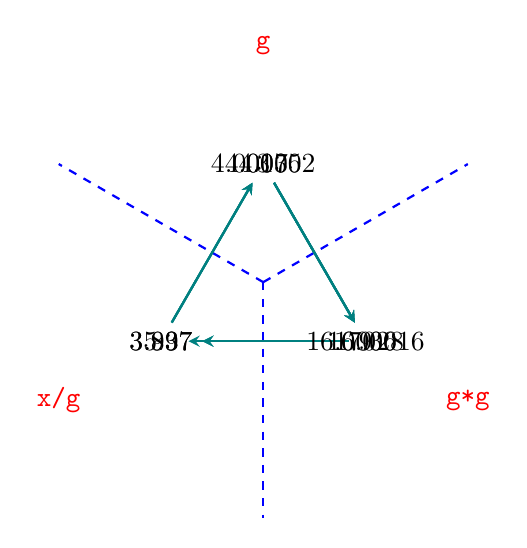
\begin{tikzpicture}[
				%every node/.style={minimum size=1cm, font=\footnotesize, inner sep=1pt},
				con/.style={thick, -stealth, Teal},
				]
				\draw[dashed, thick, Blue] (0,0) edge (30:3) edge (150:3) edge (270:3);
				\node[Red, font=\tt] at (90:3) {g};
				\node[Red, font=\tt] at (-30:3) {g*g};
				\node[Red, font=\tt] at (210:3) {x/g};
				\node<1-3>(1) at (90:1.5) {3};

				\node<2-3> (2) at (-30:1.5) {9};
				\draw<2>[con] (1) -- (2);
				\node<3-4>(3) at (210:1.5) {5.3};
				\draw<3>[con] (2) -- (3);
				\node<4-5>(4) at (90:1.5) {4.17};
				\draw<4>[con] (3) -- (4);

				\node<5-6>(5) at (-30:1.5) {17.36};
				\draw<5>[con] (4) -- (5);
				\node<6-7>(6) at (210:1.5) {3.837};
				\draw<6>[con] (5) -- (6);
				\node<7-8>(7) at (90:1.5) {4.0035};
				\draw<7>[con] (6) -- (7);

				\node<8-9>(8) at (-30:1.5) {16.028};
				\draw<8>[con] (7) -- (8);
				\node<9-10>(9) at (210:1.5) {3.997};
				\draw<9>[con] (8) -- (9);
				\node<10-11>(10) at (90:1.5) {4.000002};
				\draw<10>[con] (9) -- (10);

				\node<11->(11) at (-30:1.5) {16.000016};
				\draw<11>[con] (10) -- (11);
			\end{tikzpicture}
		\end{center}
	\end{columns}
\end{frame}

\begin{frame}{Delicious Recipes}
	\begin{itemize}[<+->]
		\item What comprised our recipe?
			\begin{enumerate}
				\item A sequence of simple \alert{steps}
				\item Some \alert{control flow} that specified when to execute each step
				\item Some method of determining when to \alert{stop}
			\end{enumerate}
		\item The 3 together comprise what we call an \alert{algorithm}
			\begin{itemize}
				\item Algorithms are what you use to solve your problem or accomplish your task
				\item Programming or coding is how you communicate those algorithms to the computer
			\end{itemize}
	\end{itemize}
\end{frame}

\begin{frame}{Rise of the Machine}
	\begin{itemize}
		\item Recipes can be bound or connected to a machine in a variety of ways
			\begin{itemize}
				\item Mechanical, electrical, hydraulic, etc
			\end{itemize}
		\item Computing machines (computers) fall into two overall categories depending on their capabilities
			\begin{itemize}
				\item \alert{Fixed program} computers
					\begin{itemize}
						\item Algorithm(s) hardcoded into the machine and can't be easily changed
					\end{itemize}
				\item \alert{Stored program} computers
					\begin{itemize}
						\item The machines executes \emph{and} stores instructions
					\end{itemize}
			\end{itemize}
	\end{itemize}
\end{frame}

\begin{frame}{Stored Programs}
	\begin{itemize}
		\item Some sequence of instructions is \emph{stored} inside the computer
			\begin{itemize}
				\item Generally built from a predefined set of primitive instructions. Things like:
					\begin{itemize}
						\item arithmetic
						\item logic
						\item simple tests
						\item moving around data
					\end{itemize}
			\end{itemize}
		\item Some special program (the interperter) executes each instruction in order
			\begin{itemize}
				\item Simple tests control the flow of instructions
				\item Stop when out of instructions
			\end{itemize}
	\end{itemize}
\end{frame}

\begin{frame}{How Primitive}
	\begin{itemize}
		\item<1-> Alan Turing describes with his Turing Machine that \alert{any computable} problem can be solved with 6 basic primitive operations
			\begin{itemize}
				\item There do exist problems whose solutions simply can not be computed!
			\end{itemize}
		\item<2-> The Church-Turing thesis ensures that if any machine can simulate a Turing Machine, then it is also a Turing Machine
			\begin{itemize}
				\item Said to be \alert{Turing Complete}
				\item All modern languages are Turing Complete, as well as many other things!
					\begin{itemize}
						\item \link{https://arxiv.org/pdf/1904.09828.pdf}{Magic: The Gathering} $\leftarrow$ scientific paper
						\item \link{http://aurellem.org/vba-clojure/html/total-control.html}{Pokemon Yellow} $\leftarrow$ creating a midi player from Pokemon Yellow
						\item Minecraft
						\item Excel
						\item \link{https://www.youtube.com/watch?v=uNjxe8ShM-8}{Powerpoint} $\leftarrow$ very worth watching!
						\item and \link{http://beza1e1.tuxen.de/articles/accidentally_turing_complete.html}{more}
					\end{itemize}
			\end{itemize}
		\item<3-> Modern languages have much more convenient primitives to work with
	\end{itemize}
\end{frame}
\note{This is a test.}

\begin{frame}{Communication}
	\begin{itemize}
		\item The programming language provides some set of primitive operations
			\begin{itemize}
				\item For instance \pyi{*} or \pyi{+}
			\end{itemize}
		\item We combine those with \alert{literals} to describe what we want the machine to do
			\begin{itemize}
				\item Examples would be numbers: \pyi{25}, or strings of characters: \pyi{"fishsticks"}.
			\end{itemize}
		\item Legal combinations of literals and operations are call \alert{expressions}
			\begin{itemize}
				\item But what constitutes ``legal''?
			\end{itemize}
	\end{itemize}
\end{frame}

\begin{frame}{Aspects of Languages}
	\begin{itemize}
		\item Any language, English or Python, has rules about how you can combine its constituent parts
		\item \alert{Syntax} defines how various elements or parts must be arranged to be well formed.
			\begin{itemize}
				\item In English, proper sentences have subject and predicate, or generally {\tt<noun>}, {\tt<verb>}, {\tt<noun>}.
					\begin{itemize}
						\item ``Billy cow house'' $\leftarrow$ not syntactically valid
						\item ``Billy runs home'' $\leftarrow$ syntactically valid
					\end{itemize}
				\item In Python, we commonly have {\tt<literal>}, {\tt<operation>}, {\tt<literal>}
					\begin{itemize}
						\item \pyi{7"hi"} $\leftarrow$ not syntactically valid
						\item \pyi{7*12} $\leftarrow$ syntactically valid
					\end{itemize}
			\end{itemize}
	\end{itemize}
\end{frame}

\begin{frame}{Syntax is not enough}
	\begin{itemize}
		\item It is totally possible to have syntactically valid language that still doesn't make sense or have meaning:
			\begin{itemize}
				\item ``Trees drops branches.''
			\end{itemize}
		\item \alert{Static semantics} defines which syntactically valid expressions have meaning.
			\begin{itemize}
				\item \pyi{12+5} $\leftarrow$ syntactically valid and valid static semantics
				\item \pyi{12+"hi"} $\leftarrow$ syntactically valid but static semantic error
			\end{itemize}
	\end{itemize}
\end{frame}

\begin{frame}{Python $>$ English}
	\begin{itemize}
		\item \alert{Semantics} is the meaning associated with a syntactically correct string of symbols with no static semantic errors.
			\begin{itemize}
				\item In English, we often can have sentences with multiple meanings:
					\begin{itemize}
						\item ``Flying planes can be dangerous.''
						\item ``I can not praise this student too highly.''
					\end{itemize}
				\item In programming, an expression will only have a single meaning
					\begin{itemize}
						\item But it may be different that the programmer intended!
					\end{itemize}
			\end{itemize}
	\end{itemize}
\end{frame}

\begin{frame}{Where everything breaks\ldots}
	\begin{itemize}
		\item Syntax errors:
			\begin{itemize}
				\item happen often and are easily caught and fixed
			\end{itemize}
		\item Static semantic errors
			\begin{itemize}
				\item Some languages will check before running
				\item Python doesn't do much before but will check and can catch some while running
			\end{itemize}
		\item No semantic errors, but different meaning than intended
			\begin{itemize}
				\item Program crashes and stops running
				\item Program runs forever
				\item Program gives answer but incorrect or different than expected
			\end{itemize}
	\end{itemize}
\end{frame}





\end{document}

